\documentclass[twoside,11pt]{article}

% Any additional packages needed should be included after jmlr2e.
% Note that jmlr2e.sty includes epsfig, amssymb, natbib and graphicx,
% and defines many common macros, such as 'proof' and 'example'.
%
% It also sets the bibliographystyle to plainnat; for more information on
% natbib citation styles, see the natbib documentation, a copy of which
% is archived at http://www.jmlr.org/format/natbib.pdf

\usepackage{jmlr2e}
\usepackage{minted}
\usepackage[demo]{graphicx}
\usepackage{caption}
\usepackage{subcaption}
\usepackage[colorinlistoftodos]{todonotes}

% Definitions of handy macros can go here

\newcommand{\dataset}{{\cal D}}
\newcommand{\fracpartial}[2]{\frac{\partial #1}{\partial  #2}}

% Heading arguments are {volume}{year}{pages}{submitted}{published}{author-full-names}

\jmlrheading{1}{2000}{1-48}{4/00}{10/00}{Marina Meil\u{a} and Michael I. Jordan}

% Short headings should be running head and authors last names

\ShortHeadings{Learning with Mixtures of Trees}{Meil\u{a} and Jordan}
\firstpageno{1}

\begin{document}

\title{Metric-learn: Metric Learning in Python}

\author{\name Marina Meil\u{a} \email mmp@stat.washington.edu \\
       \addr Department of Statistics\\
       University of Washington\\
       Seattle, WA 98195-4322, USA
       \AND
       \name Michael I.\ Jordan \email jordan@cs.berkeley.edu \\
       \addr Division of Computer Science and Department of Statistics\\
       University of California\\
       Berkeley, CA 94720-1776, USA}

\editor{Leslie Pack Kaelbling}

\maketitle

\begin{abstract}%   <- trailing '%' for backward compatibility of .sty file
TODO
\end{abstract}

\begin{keywords}
  Machine Learning, Python, Metric Learning, Scikit-learn
\end{keywords}

\section{Introduction}

\begin{itemize}
    \item Metric learning
    \item Importance of supporting the classic ML workflows for model selection, model evaluation, pipelining with other estimators etc, via sklearn. makes metric-learn stands out from other packages
    in particular in the case of weakly supervised algorithms
\end{itemize}

% Acknowledgements should go at the end, before appendices and references

\section{Overview of the Package}
\texttt{metric-learn} is  a
\todo[inline]{GitHub repo, PyPi, mention current release, license}
\texttt{metric-learn} only relies on core libraries from the SciPy ecosystem: \texttt{numpy}, \texttt{scipy}, and \texttt{scikit-learn}. An optional dependency with \texttt{skggm} (\cite{skggm}) can be installed in order to use a more stable solver when using the LSML algorithm from the package.
It can be installed from the Python Package Index (PyPI), on python 2.7 and 3.5 or later.  The source code is available at \url{http://github.com/metric-learn/metric-learn}. The development is collaborative and open to all. The code is free of use, provided under the MIT licence. The current realease is 0.5.0. It includes many refactoring including the ones described in the paper, that improve scikit-learn compatibility.

\section{Available algorithms}

\texttt{metric-learn} contains most of the highly cited Mahalanobis metric learning algorithms. 

\subsection{Mahalanobis metric learning}
Mahalanobis learning algorithms learn a 


Here is a list of the algorithms contained in \texttt{metric-learn}:
\subsection{Supervised Metric Learning algorithms}
Supervised algorithms learns a metric that brings closer together points from the same class and spreads further away points from a different class.
\begin{itemize}
    \item NCA: Neighborhood Components Analysis
    \item LMNN: Large Margin Nearest Neighbors
    \item RCA: Relative Components Analysis
    \item LFDA: Local Fisher Discriminant Analysis
\end{itemize}
\subsection{Weakly Supervised Metric Learning algorithms}
Weakly Supervised algorithms use less information than the previous algorihtms: they only take tuple of points and possibly a corresponding label. See below for more concrete examples of algorithms learning on tuples.
    \subsubsection{Pairs Learners} 
    Pairs learners take as input pair of points, and a corresponding label indicating whether the two points are similar or not. They will learn a metric that brings points from a similar pair closer together, and points from a dissimilar pair further away from each other.
    \begin{itemize}
        \item MMC: Mahalanobis Metric for Clustering
        \item SDML: Sparse High-Dimensional Metric Learning (SDML)
        \item ITML: Information Theoretic Metric Learning (ITML)
    \end{itemize}
    
    \begin{figure}[H]
\centering
\begin{subfigure}{.5\textwidth}
  \centering
  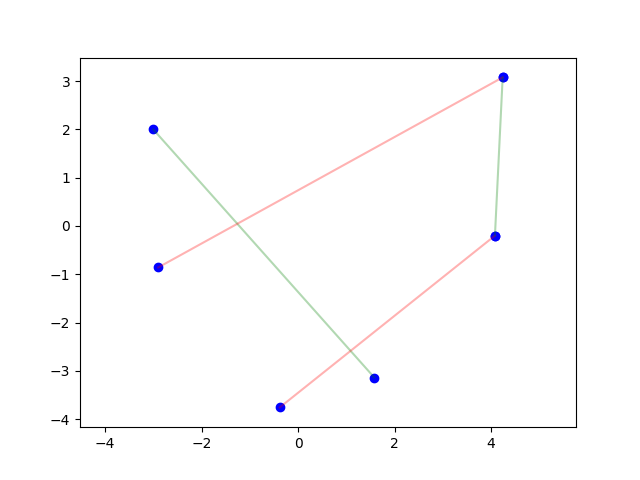
\includegraphics[width=.8\linewidth]{pairs_without_metric.png}
  \caption{Original points, before metric learning}
  \label{fig:sub1}
\end{subfigure}%
\begin{subfigure}{.5\textwidth}
  \centering
  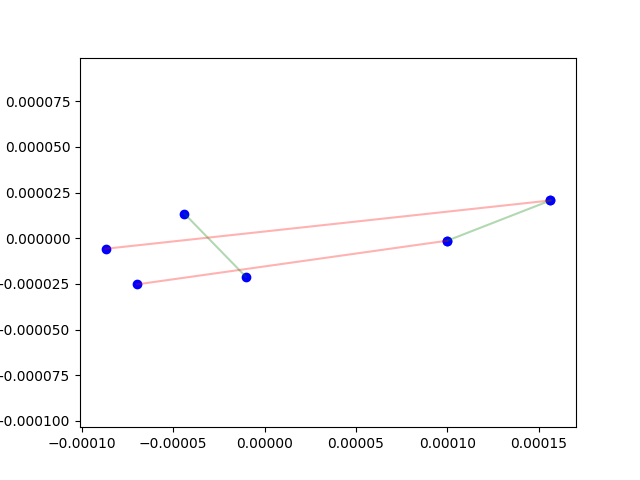
\includegraphics[width=.8\linewidth]{pairs_with_metric.png}
  \caption{Points after metric learning (ITML)}
  \label{fig:sub2}
\end{subfigure}
\caption{Metric learning with pairwise constraints}
\label{fig:test}
\end{figure}
    
    \subsubsection{Quadruplets Learners}
    Quadruplets learners take as input quadruplets of points. They learn a metric that brings the two first points of each quadruplet closer than the two last points are.
    \begin{itemize}
        \item LSML: Metric Learning from Relative Comparisons by Minimizing Squared Residual
    \end{itemize}

\todo[inline]{Mention and link documentation}

\textbf{Documentation} A detailed documentation, including installation guidelines, the description of the algorithms and the API, as well as example of use done with \texttt{sphinx-gallery}, is available at \url{https://metric-learn.github.io/metric-learn/}. It also includes \texttt{intersphinx} bindings for more efficient navigation through the documentation of the whole \texttt{scipy} ecoystem. 

\todo[inline]{Code example to showcase usage, potentially with compelling visualization?}

\todo[inline]{what about four plots: two plots for supervised metric learning: before and after learning the metric (classes are the colors of the points), and two plots for weakly supervised metric learning (same) (with red segments for negative constraints and green for positive constraints)}

One of the main advantage of metric-learn is its possibility to be used with 

\begin{minted}{python}
from metric_learn import MMC
pairs = np.array([[[1.2, 3.2], [2.3, 5.5]],
                  [[4.5, 2.3], [2.1, 2.3]]])
y_pairs = np.array([1, -1])
mmc = MMC(random_state=42)
mmc.fit(pairs, y_pairs)
mmc.predict(pairs)
\end{minted}

\section{Software Architecture}

\todo[inline]{API: I think we want to insist on this}

\texttt{metric-learn}'s API is designed to be fully compatible with \texttt{scikit-learn} API \cite{scikit-learn}. \texttt{metric-learn} includes different types of algorithms depending on the type of information we want to use to learn the metric. (i) Supervised metric learning algorithms take as an input sample and labels like any supervised learning algorithm, and they will learn a metric that embeds points from the same class closer to each other, and points from a different class further away from each other. (ii) Weakly supervised learning algorithms take as an input tuples of points, and a possible label for the tuple. For example, pairs learners take pairs of points and a label indicating whether the two points are similar (which we want the learned metric to bring closer together) or dissimilar (which we want the learned metric to push away from each other). The API of \texttt{metric-learn} is made so as to allow for the possible development of other types of supervision on tuples. Algorithms that are trained in a supervised way are regular \texttt{Transformers}, just like \texttt{scikit-learn}'s \texttt{LinearDiscriminantAnalysis} for instance. On the other hand, weakly supervised learning algorithms are similar to \texttt{scikit-learn} classifiers, but with input data \texttt{X, y} being tuples and labels of tuples instead of points, i.e. they \texttt{fit} on tuples, that can be represented as 3D arrays, and have a \texttt{predict} method, that gives a prediction for each given tuple. Tuples can be pairs or quadruplets, depending on the specific algorithm used. For instance, \texttt{metric-learn} contains some algorithms that learn on pairs of points and the according labels. 

\begin{minted}{python}
from metric_learn import MMC
pairs = np.array([[[1.2, 3.2], [2.3, 5.5]],
                  [[4.5, 2.3], [2.1, 2.3]]])
y_pairs = np.array([1, -1])
mmc = MMC(random_state=42)
mmc.fit(pairs, y_pairs)
mmc.predict(pairs)
\end{minted}


This allows to use out of the box \texttt{scikit-learn}'s scoring functions, and therefore all routines for model selection, including the \texttt{GridSearchCV} object. 

\begin{minted}{python}
from sklearn.model_selection import GridSearchCV
grid = {'init': ['random', 'identity', 'covariance']}
model = GridSearchCV(mmc, grid)
model.fit(pairs, y_pairs)
\end{minted}

More details on the 3D array thing: 

At the core of \texttt{metric-learn} is the format of input tuples. This format is what allows all these API choices. While a classical input array \texttt{X} in \texttt{scikit-learn} has shape \texttt{(n\_samples, n\_features)}, an array of tuples has shape \texttt{(n\_tuples, t, n\_features)}, where \texttt{t} is the number of elements in a tuple (e.g. 2 for pairs).

Note that \texttt{scikit-learn} accepts arrays in a broad sense, in what they call "array-like" objects. \texttt{metric-learn} too accepts "tuple-like" objects.


Image: a classical array of samples X
an array of pairs of X X[np.array([[1, 2], [3, 4], [2, 1]])]


\todo[inline]{CI and test coverage}

The quality of the code is ensured by an intensive test coverage of 96\%. Every new contribution to the code is automatically checked by a continuous integration platform that ensures a minimal test coverage of the added code, and an minimal variation in test coverage of the overall code. 

Contributions: This allows easy contribution for incoming developers, which can have their code automatically checked. What is more, they can instantiate their algorithm as an instance of Metric learner, to benefit from all the methods of it, and help scikit-learn compatibility. 

\section{Conclusion}

mention future developments? scalability, more algorithms, etc

scalability: 
- support stochastic solvers
- support sparsity
- form pairs on the fly and do some computations by batch

more algorithms:
- algorithms on triplets
- algorithms for high dimensional data

- toy datasets

improved CI
- pep8

\acks{TODO}

 The quality of comparison to previous (if any) related implementations, w.r.t. run-time, memory requirements, features, to explain that significant progress has been made. 

% Manual newpage inserted to improve layout of sample file - not
% needed in general before appendices/bibliography.

\bibliography{metric-learn-jmlr}

\end{document}